\chapter{از کوانتیزاسیون تا \lr{k-means}}

\section{تابع هدف پایه}

برای مجموعه‌داده‌ی $\mathcal{X}=\{x_1,\ldots,x_n\}\subset\mathbb{R}^d$ و
افراز $\mathcal{S}=\{S_1,\ldots,S_k\}$، تابع هدف رایج \lr{k-means} برابر است با
\begin{equation}
    \Phi(\mathcal{S})=\sum_{i=1}^{k}\sum_{x\in S_i}\lVert x-\mu_i\rVert_2^2,
    \qquad
    \mu_i=\frac{1}{|S_i|}\sum_{x\in S_i}x.
    \label{eq:kmeans}
\end{equation}
دو تصمیم اصلی الگوریتم عبارت‌اند از انتساب هر نقطه به یک خوشه و محاسبه‌ی
نماینده‌ی آن خوشه. برای فاصله، مربع فاصله‌ی اقلیدسی و برای انتخاب نماینده‌ی یک
خوشه، میانگین مختصات نقاط آن در نظر گرفته است.

\section{روش مک‌کوئین}

مقاله‌ی مک‌کوئین در سال ۱۹۶۷ اصطلاح \lr{k-means} را رواج داد
\cite{macqueen1967}، هرچند خود مقاله تصریح می‌کند که پیش‌تر فرایندی
از این نوع  به‌کار برده شده بود. فرمولبندی مک‌کوئین جمعیتی است: داده از توزیع
احتمال $p$ می‌آید و برای افراز $S_1,\ldots,S_k$، میانگین \underbar{شرطی} خوشه‌ی $i$
به‌صورت
\begin{equation}
    u_i=\frac{\int_{S_i}z\,dp(z)}{p(S_i)}
\end{equation}
تعریف می‌شود. واژه‌ی «شرطی» به شرط $z\in S_i$ اشاره دارد. استفاده از انتگرال
در این مقاله و استفاده از دو جمع در رابطه‌ی \ref{eq:kmeans} تفاوتی بنیادی نیست اما نکته‌ی جالب توجهی به نظر می‌رسد.

\subsection{الگوریتم برخط}

در الگوریتم اصلی، $k$ مشاهده‌ی نخست به‌عنوان مراکز اولیه انتخاب می‌شوند و
وزن هر مرکز برابر یک قرار می‌گیرد. این مقداردهی اولیه را نباید کاملاً غیرتصادفی دانست و نتیجه به ترتیب
ورود داده‌ها وابسته است. مشاهده‌ی جدید $z_{n+k}$ به نزدیک‌ترین مرکز نسبت
داده می‌شود. در حالت تساوی فاصله، مرکز با شماره‌ی کوچک‌تر انتخاب می‌شود.
اگر نقطه به خوشه‌ی $i$ افزوده شود،
\begin{equation}
    x_i^{n+1}=
    \frac{w_i^n x_i^n+z_{n+k}}{w_i^n+1},
    \qquad
    w_i^{n+1}=w_i^n+1,
    \label{eq:macqueen-update}
\end{equation}
و سایر مراکز و وزن‌ها ثابت می‌مانند. این همان به‌روزرسانی میانگین
است ولی به ذخیره‌ی تمام نقاط پیشین نیاز ندارد.

در انتهای مقاله، یک مثال مستطیل‌شکل به عنوان نمونه آورده شده تا نمایانگر حالتی باشد که این روش به انتخاب یک خوشه‌بندی نامناسب (البته به صورت محلی بهین) میپردازد.
نمونه‌ی چهار رأس یک مستطیل کمی کشیده،
این محدودیت را روشن می‌کند. برای $k=2$، الگوریتم ممکن است به افراز افقی
شکل \ref{fig:macqueen-rectangle} برسد، درحالی‌که افراز عمودی هزینه‌ی
کم‌تری دارد.

\begin{figure}[H]
    \centering
    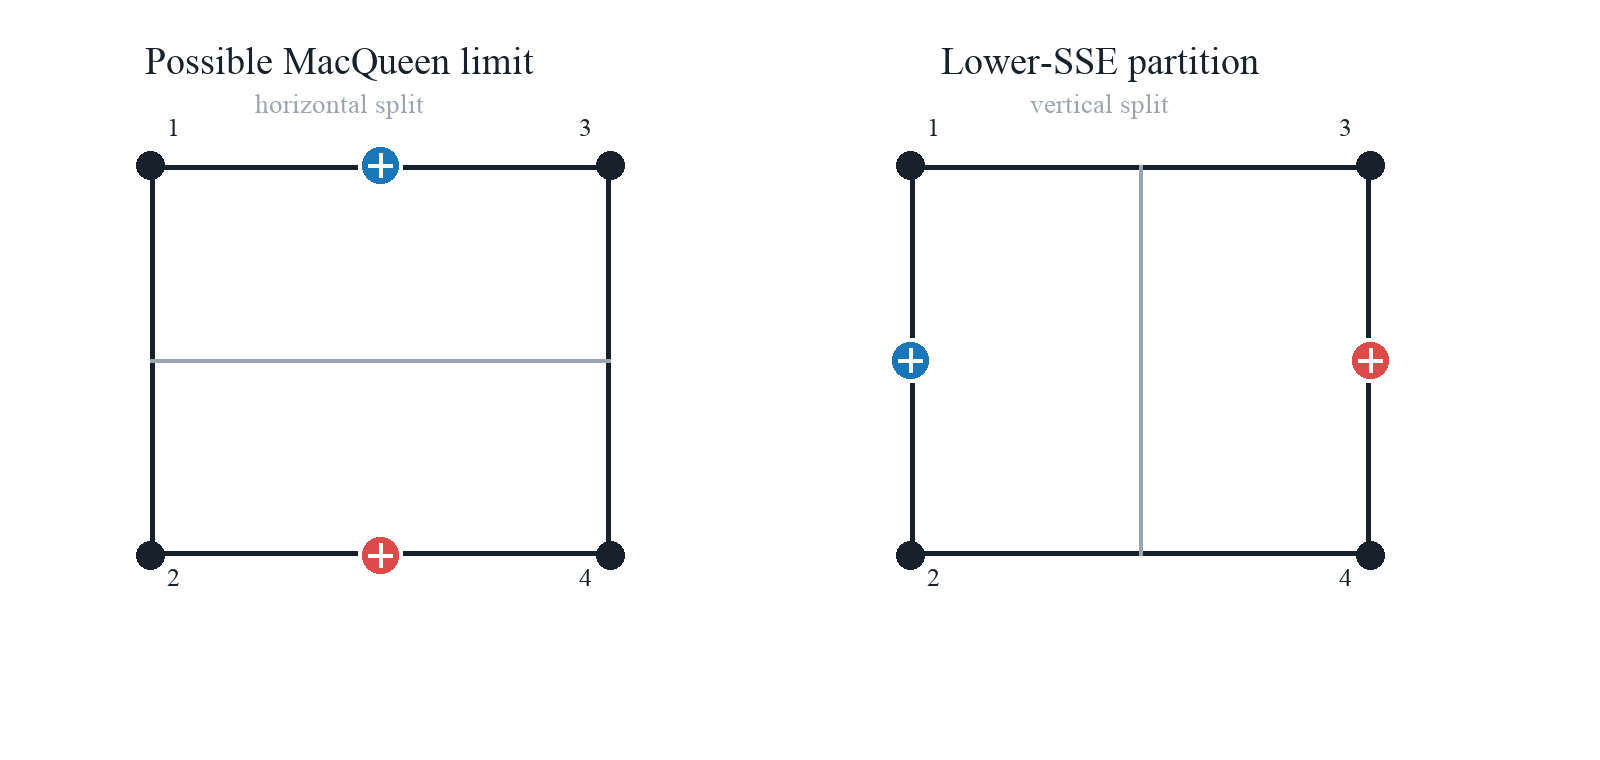
\includegraphics[width=.92\textwidth]{Figures/macqueen_rectangle.png}
    \caption{نمونه‌ی مستطیل در مقاله‌ی مک‌کوئین؛ یک حد ممکن در سمت چپ و افراز
        کم‌هزینه‌تر در سمت راست.}
    \label{fig:macqueen-rectangle}
\end{figure}

\subsection{نسخه‌ی دسته‌ای و تغییر تعداد مراکز}

بخش ۳٫۶ مقاله یک روش دسته‌ای را توصیف می‌کند: از یک افراز آغاز می‌شود،
میانگین همه‌ی خوشه‌ها هم‌زمان محاسبه می‌شود، تمام نقاط دوباره به نزدیک‌ترین
میانگین نسبت داده می‌شوند و این دو گام تکرار می‌شوند. برخلاف نسخه‌ی برخط،
در اینجا کل مجموعه‌داده در هر دور بازبینی می‌شود. روی داده‌ی متناهی، واریانس
درون‌خوشه‌ای کاهش می‌یابد و فرایند پس از تعداد متناهی گام متوقف می‌شود.

مک‌کوئین همچنین دو آستانه‌ی $C$ و $R$ را برای تغییر  تعداد مراکز
پیشنهاد می‌کند: دو مرکز با فاصله‌ی کمتر از $C$ ادغام
می‌شوند و نقطه‌ای با فاصله‌ی بیش از $R$ از نزدیک‌ترین مرکز، خود به مرکز
جدید تبدیل می‌شود.

\section{لوید و کوانتیزاسیون کمترین مربعات}

مقاله‌ی لوید
\cite{lloyd1982} ابتدا در سال ۱۹۵۷ در آزمایشگاه بل نوشته شد و در سال
۱۹۸۲ انتشار یافت. هدف، نمایش نمونه‌های ولتاژ با تعداد محدودی مقدار
بازسازی‌شده و کمینه کردنِ متوسطِ نویز کوانتیزاسیون بود.

\begin{table}[H]
    \centering
    \caption{ترجمه‌ی اصطلاحات لوید به زبان خوشه‌بندی}
    \begin{tabular}{p{.38\textwidth}p{.48\textwidth}}
        \toprule
        لوید                                & \lr{k-means}                           \\
        \midrule
        نمونه‌های ولتاژ                      & نقاط داده                              \\
        بازه‌ها یا زیرمجموعه‌های کوانتیزاسیون & خوشه‌ها                                 \\
        مقادیر کوانتیزه $q_a$               & مراکز یا میانگین‌های خوشه               \\
        نویز کوانتیزاسیون                   & مجموع مربعات خطا                   \\
        کمینه کردن متوسط نویز          & کمینه کردن فاصله‌ی مربع‌شده‌ی مورد انتظار \\
        \bottomrule
    \end{tabular}
\end{table}

\section{خروجی تعاملی فصل}

فایل \lr{interactive/macqueen-vs-lloyd.html} دو روش را روی یک داده‌ی مشترک
کنار هم نمایش می‌دهد. در سمت مک‌کوئین، هر گام فقط یک نقطه و یک میانگین را تغییر می‌دهد؛ در سمت لوید، انتساب برای همه‌ی نقاط صورت گرفته و سپس همه‌ی مراکز
به‌صورت دسته‌ای به‌روز می‌شوند.